\section{Use Cases Model}
\label{sec:Use Cases Model}
% Descirbes the functional requirements, mostly non-functional. During incepeion, the names of most use cases will be indentified, and perhapss 10% of teh use cases will be analyzed in detail.
% 
\subsection{Actors}
\label{subsec:Actors}
\begin{table}[htp]
  \definecolor{tcA}{rgb}{0.862745,0.862745,0.862745}
  \begin{tabular}[t]{|l|l|l|}\hline
  % use packages: color,colortbl
	  \rowcolor{tcA}
	  Actor 		& Typ 		& Beschreibung \\\hline
	  User		 	& primary 	& Interagiert mit dem System. \\\hline
	  Operating System 	& supporting 	& Dient dem System beim Zugriff auf das Dateisystem. \\\hline
	  Algorithm Developer 	& offstage 	& Entwickler von Algorithmen. \\\hline
  \end{tabular}
  \caption{Actors}
  \label{tab:actors}
\end{table}

% 
\subsection{Use Cases Diagram}
\label{subsec:Use Cases Diagram}
\begin{figure}[H]
    \centering
    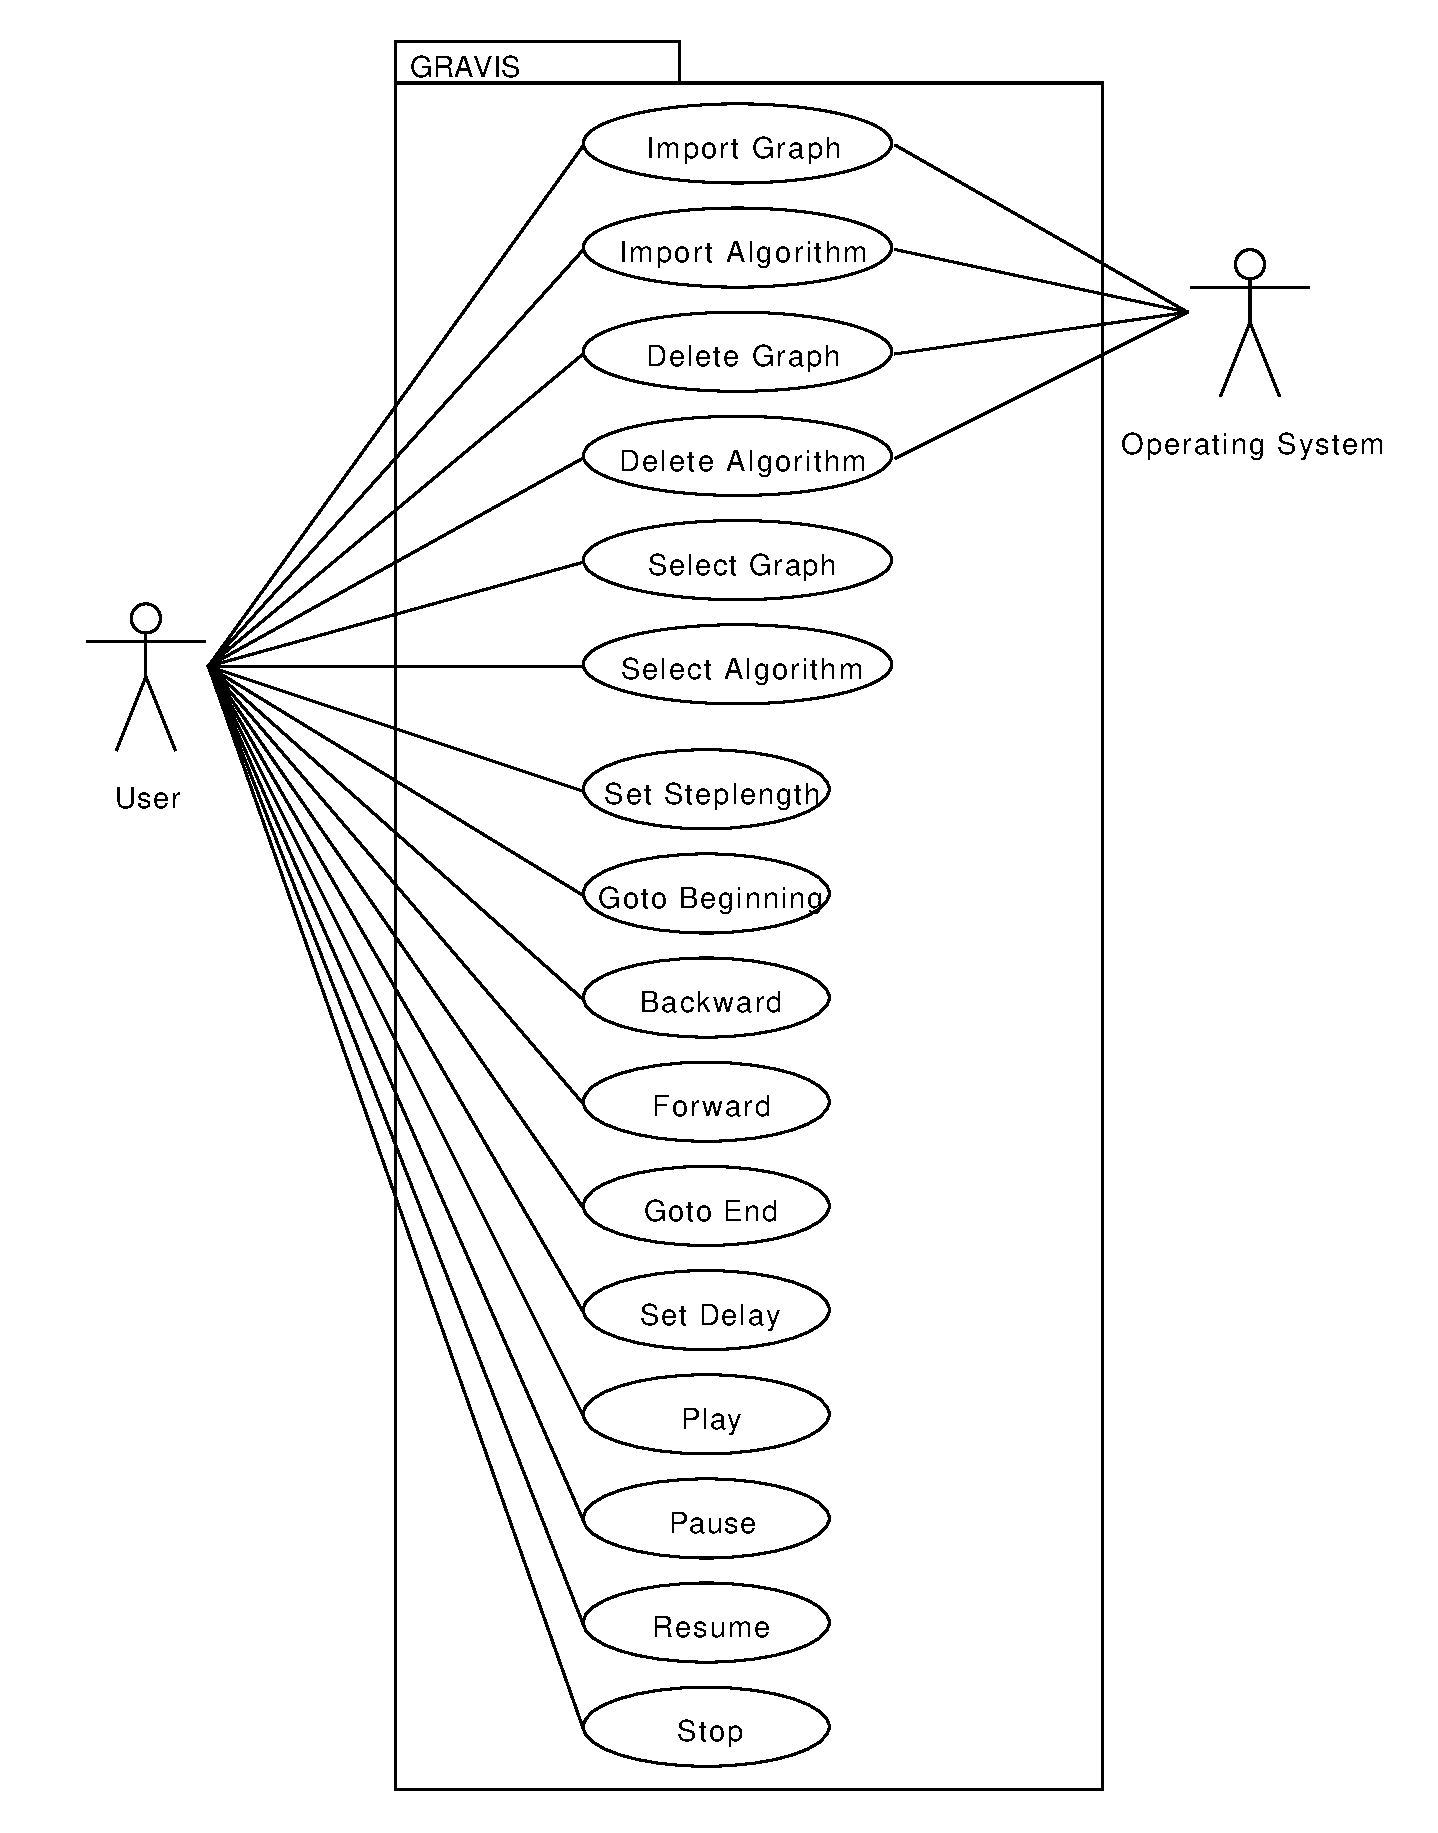
\includegraphics[scale=0.5]{diagrams/use-cases-diagram.pdf}
    \caption{Use Cases Diagram}
    \label{fig:use_cases_diagram}
\end{figure}
% 
\subsection{Use Cases in Brief Format}
\label{subsec:Use Cases in Brief Format}
% - All the use-cases of the application you discover, which have to be written in brief format;
\begin{description}
  \item[Import Graph:] Der User kann einen neuen Graphen importieren.

  (Ausgearbeitetes Format siehe Seite~\pageref{uc:Import Graph})

  \item[Import Algorithm:] Der User kann einen neuen Algorithmus importieren.

  (Ausgearbeitetes Format siehe Seite~\pageref{uc:Import Algorithm})

  \item[Delete Graph:] Der User kann einen importierten Graphen l\"oschen.

  (Ausgearbeitetes Format siehe Seite~\pageref{uc:Delete Graph})

  \item[Delete Algorithm:] Der User kann einen importierten Algorithmus l\"oschen.

  (Ausgearbeitetes Format siehe Seite~\pageref{uc:Delete Algorithm})

  \item[Select Graph:] Der User kann einen Graphen ausw\"ahlen.

  (Ausgearbeitetes Format siehe Seite~\pageref{uc:Select Graph})

  \item[Select Algorithm:] Der User kann einen Algorithmus ausw\"ahlen.

  (Ausgearbeitetes Format siehe Seite~\pageref{uc:Select Algorithm})

  \item[Set Steplength:] Der User kann f\"ur die Visualisierung die Anzahl Traversierungsschritte pro Bild einstellen.

  \item[Forward:] Der User kann in der Step-by-Step-Visualisierung ein Bild vorw\"arts gehen.

  \item[Backward:] Der User kann in der Step-by-Step-Visualisierung ein Bild r\"uckw\"arts gehen.

  \item[Goto Beginning:] Der User kann in der Step-by-Step-Visualisierung an das Ende springen.

  \item[Goto End:] Der User kann in der Step-by-Step-Visualisierung an den Anfang springen.

  \item[Set Delay:] Der User kann f\"ur die animierte Visualisierung das Zeitintervall zwischen zwei Bildern einstellen.

  \item[Play:] Der User kann die animierte Visualisierung starten.

  \item[Pause:] Der User kann die animierte Visualisierung pausieren.

  \item[Resume:] Der User kann die pausierte animierte Visualisierung wieder aktivieren.

  \item[Stop:] Der User kann die animierte Visualisierung anhalten.
\end{description}
% 
\subsection{Use Cases in Fully Dressed Format}
\label{subsec:Use Cases in Fully Dressed Format}
Die sechs UC \textit{Import Graph}, \textit{Import Algorithm}, \textit{Delete Graph}, \textit{Delete Algorithm}, \textit{Select Graph} und \textit{Select Algorithm} werden im ausgearbeiteten Format erl\"autert. F\"ur diese UC gilt:
\begin{itemize}
  \item Scope: System-wide
  \item Level: User-goal
  \item Primary Actor: User
\end{itemize}
\newpage
% 
\begin{usecase}{Import Graph}
    \preconditions{
	    \item Die Benutzerschnittstelle zur Befehlswahl ist aktiv.
	    \item Die Dateistruktur des Betriebssystems ist zug\"anglich.
	    \item Auf die zu importierende Datei sind mindestens Leserechte gesetzt.
    }
    \postconditions{
	    \item Der Parameter steht dem System zur weiteren Verarbeitung zur Verf\"ugung.
	    \item Der Parameter steht dem User in der Parameterliste zur Auswahl bereit.
            \item Die Parameterlisten wurden auf Default-Werte gesetzt.
	    \item Die Parameterlisten der Benutzerschnittstellen wurden aktualisiert.
	    \item Der Graph wurde durch das System ausgew\"ahlt und im GUI dargestellt.
    }
    \mainsuccess{
	    \item Der User startet den Graph-Import.
	    \item Der User wird dazu aufgefordert, den Pfad und den Dateinamen einer Datei anzugeben oder den Vorgang abzubrechen.
	    \item Die angegebene Datei wird in die Dateistruktur des Systems kopiert.
	    \item Die angegebene Datei wird durch das System auf Kompatibilit\"at gepr\"uft.
	    \item Der zu importierte Graph wird zur Graph-Parameterliste hinzugef\"ugt.
	    \item Der Graph wird durch das System in der Graph-Parameterliste ausgew\"ahlt (siehe \textit{UC Select Graph}, Seite~\pageref{uc:Select Graph}.
    }
%     \newpage
%     \hline \\ [-1.3ex]
%     \extensions{
% 	    \item[1.a]
% 		    \begin{enumerate}
% 			\item Das Starten des Vorganges \textbf{schl\"agt fehl}.
% 			\item Eine Fehlermeldung wird ausgegeben.
% 		    \end{enumerate}
% 	    \item[2.a]
% 		    \begin{enumerate}
% 			\item Der User \textbf{bricht den Vorgang ab}.
% 		    \end{enumerate}
% 	    \item[2.b]
% 		    \begin{enumerate}
% 			\item Die angegebene Datei kann \textbf{nicht gefunden} werden.
% 			\item Eine Fehlermeldung wird ausgegeben.
% 			\item Dem User wird widerum die M\"oglichkeit gegeben, den Pfad und den Dateinamen einer Datei anzugeben oder den Vorgang abzubrechen (Rekursion).
% 		    \end{enumerate}
% 	    \item[3.a]
% 		    \begin{enumerate}
% 			\item Die angegebene Datei \textbf{kann nicht} in die Dateistruktur des Systems \textbf{kopiert werden}.
% 			\item Eine Fehlermeldung wird ausgegeben.
% 		    \end{enumerate}
% 	    \item[4.a]
% 		    \begin{enumerate}
% 			\item Die angegebene Datei ist \textbf{nicht kompatibel}.
% 			\item Die kopierte Datei wird aus der Dateistruktur des Systems gel\"oscht.
% 			\item Eine Fehlermeldung wird ausgegeben.
% 		    \end{enumerate}
% 	    \item[5.a]
% 		    \begin{enumerate}
% 			\item Der Name des importierten Graphen \textbf{kann nicht zur Parameterliste hinzugef\"ugt werden}.
% 			\item Die kopierte Datei wird aus der Dateistruktur des Systems gel\"oscht.
% 			\item Eine Fehlermeldung wird ausgegeben.
% 		    \end{enumerate}
% 	    \item[6.a]
% 		    \begin{enumerate}
% 			\item siehe \textit{UC Select Graph}, Seite~\pageref{uc:Select Graph} resp. \textit{UC Select Algorithm}, Seite~\pageref{uc:Select Algorithm}.
% 		    \end{enumerate}
%     }
\end{usecase}
\newpage 
% 
\begin{usecase}{Import Algorithm}
    \preconditions{
	    \item Die Benutzerschnittstelle zur Befehlswahl ist aktiv.
	    \item Die Dateistruktur des Betriebssystems ist zug\"anglich.
	    \item Auf die zu importierende Datei sind mindestens Leserechte gesetzt.
    }
    \postconditions{
	    \item Der Parameter steht dem System zur weiteren Verarbeitung zur Verf\"ugung.
	    \item Die Graph-Parameterliste wurde aktualisiert.
	    \item Die Parameterlisten wurden auf Default-Werte gesetzt.
	    \item Die Parameterlisten der Benutzerschnittstellen wurden aktualisiert.
    }
    \mainsuccess{
	    \item Der User startet den Algorithmus-Import.
	    \item Der User wird dazu aufgefordert, den Pfad und den Dateinamen einer Datei anzugeben oder den Vorgang abzubrechen.
	    \item Die angegebene Datei wird in die Dateistruktur des Systems kopiert.
	    \item Die Datei wird durch das System auf Kompatibilit\"at gepr\"uft.
	    \item Der Name des importierten Parameters wird zur Parameterliste der entsprechenden Benutzerschnittstelle hinzugef\"ugt.
    }
%     \newpage
%     \hline \\ [-1.3ex]
%     \extensions{
% 	    \item[1.a]
% 		    \begin{enumerate}
% 			\item Das Starten des Vorganges \textbf{schl\"agt fehl}.
% 			\item Eine Fehlermeldung wird ausgegeben.
% 		    \end{enumerate}
% 	    \item[2.a]
% 		    \begin{enumerate}
% 			\item Der User \textbf{bricht den Vorgang ab}.
% 		    \end{enumerate}
% 	    \item[2.b]
% 		    \begin{enumerate}
% 			\item Die angegebene Datei kann \textbf{nicht gefunden} werden.
% 			\item Eine Fehlermeldung wird ausgegeben.
% 			\item Dem User wird widerum die M\"oglichkeit gegeben, den Pfad und den Dateinamen einer Datei anzugeben oder den Vorgang abzubrechen (Rekursion).
% 		    \end{enumerate}
% 	    \item[3.a]
% 		    \begin{enumerate}
% 			\item Die angegebene Datei \textbf{kann nicht} in die Dateistruktur des Systems \textbf{kopiert werden}.
% 			\item Eine Fehlermeldung wird ausgegeben.
% 		    \end{enumerate}
% 	    \item[4.a]
% 		    \begin{enumerate}
% 			\item Die angegebene Datei ist \textbf{nicht kompatibel}.
% 			\item Die Datei wird aus der Dateistruktur des Systems gel\"oscht.
% 			\item Eine Fehlermeldung wird ausgegeben.
% 		    \end{enumerate}
% 	    \item[5.a]
% 		    \begin{enumerate}
% 			\item Der Name des importierten Parameters \textbf{kann nicht zur Parameterliste hinzugef\"ugt werden}.
% 			\item Der importierte Parameter wird aus dem Arbeitsspeicher gel\"oscht.
% 			\item Die importierte Datei wird aus der Dateistruktur des Systems gel\"oscht.
% 			\item Eine Fehlermeldung wird ausgegeben.
% 		    \end{enumerate}
% 	    \item[6.a]
% 		    \begin{enumerate}
% 			\item siehe \textit{UC Select Graph}, Seite~\pageref{uc:Select Graph} resp. \textit{UC Select Algorithm}, Seite~\pageref{uc:Select Algorithm}.
% 		    \end{enumerate}
%     }
\end{usecase}
\newpage 
% 
\begin{usecase}{Delete Graph}
    \preconditions{
	    \item Die Benutzerschnittstelle zur Befehlswahl ist aktiv.
	    \item Die Dateistruktur des Betriebssystems ist zug\"anglich.
	    \item Auf die zu l\"oschende Datei sind Schreibrechte gesetzt.
    }
    \postconditions{
	    \item Die Datei wurde aus dem System gel\"oscht.
	    \item Die Graph-Parameterliste wurde aktualisiert.
	    \item Die Parameterlisten wurden auf Default-Werte gesetzt.
	    \item Die Parameterlisten der Benutzerschnittstellen wurden aktualisiert.
    }
    \mainsuccess{
	    \item 
    }
%     \hline \\ [-1.3ex]
%     \extensions{
% 	    \item[1.a]
% 		    \begin{enumerate}
% 			\item 
% 		    \end{enumerate}
%     }
\end{usecase}
\newpage 
% 
\begin{usecase}{Delete Algorithm}
    \preconditions{
	    \item Die Benutzerschnittstelle zur Befehlswahl ist aktiv.
	    \item Die Dateistruktur des Betriebssystems ist zug\"anglich.
	    \item Auf die zu l\"oschende Datei sind Schreibrechte gesetzt.
    }
    \postconditions{
	    \item Die Datei wurde aus dem System gel\"oscht.
	    \item Die Algorithm-Parameterliste wurde aktualisiert.
	    \item Die Parameterlisten wurden auf Default-Werte gesetzt.
	    \item Die Parameterlisten der Benutzerschnittstellen wurden aktualisiert.
    }
    \mainsuccess{
	    \item 
    }
%     \hline \\ [-1.3ex]
%     \extensions{
% 	    \item[1.a]
% 		    \begin{enumerate}
% 			\item 
% 		    \end{enumerate}
%     }
\end{usecase}
\newpage 
% 
\begin{usecase}{Select Graph}
    \precondition{
	    Die Benutzerschnittstelle zur Wahl eines Graphen ist aktiv.
    }
    \postconditions{
	    \item Der Graph wurde als ausgew\"ahlt markiert (\textit{selected}).
	    \item Der gew\"ahlte Graph steht als geladene Instanz zur weiteren Verarbeitung zur Verf\"ugung.
	    \item Der gew\"ahlte Graph ist visualisiert.
	    \item Die auf den Graphen anwendbaren Algorithmen wurden aktiv gesetzt (\textit{enable}).
	    \item Die Parameterlisten der Benutzerschnittstellen wurden aktualisiert.
    }
    \mainsuccess{
	    \item In der Parameterliste wird der gew\"ahlte Graph alsaktuell gesetzt.
	    \item Der vormalige Graph wird im System entladen.
	    \item Der gew\"ahlte Graph wird im System geladen.
	    \item Die auf den Graphen anwendbaren Algorithmen werden aktiv gesetzt (\textit{enable}).
	    \item Die Parameterlisten der Benutzerschnittstellen werden aktualisiert.
	    \item Der aktuelle Graph wird im Visualizer dargestellt.
    }
%     \hline \\ [-1.3ex]
%     \extensions{
% 	    \item[1.a]
% 		    \begin{enumerate}
% 			\item Das Setzen des gew\"ahlten Graphen als aktuell \textbf{schl\"agt fehl}.
% 			\item Eine Fehlermeldung wird ausgegeben.
% 		    \end{enumerate}
% 	    \item[2.a]
% 		    \begin{enumerate}
% 			\item Der vormalige Graph kann \textbf{nicht entladen} werden.
% 			\item In der Parameterliste wird der vormalige Graph als aktuell gesetzt.
% 			\item Eine Fehlermeldung wird ausgegeben.
% 		    \end{enumerate}
% 	    \item[3.a]
% 		    \begin{enumerate}
% 			\item Der gew\"ahlte Graph kann \textbf{nicht geladen} werden.
% 			\item In der Parameterliste Graph wird ein leerer Default-Wert als aktuell gesetzt.
% 			\item Eine Fehlermeldung wird ausgegeben.
% 		    \end{enumerate}
%     }
\end{usecase}
\newpage 
% 
\begin{usecase}{Select Algorithm}
    \preconditions{
	    \item Die Benutzerschnittstelle zur Wahl eines Algorithm ist aktiv.
	    \item In der Benutzerschnittstelle zur Wahl des Algorithm steht mindestens ein aktivierter Algorithm zur Auswahl zur Verf\"ugung.
    }
    \postconditions{
	    \item Der Algorithm wurde als ausgew\"ahlt markiert (\textit{selected}).
	    \item Der gew\"ahlte Algorithm wurde als Instanz geladen.
	    \item Die Parameterliste der Benutzerschnittstelle wurde aktualisiert.
            \item Der gew\"ahlte Algorithm hat eine Traversal generiert.
	    \item Das System ist zur Visualisierung der Traversal bereit.
    }
    \mainsuccess{
	    \item In der Parameterliste wird der gew\"ahlte Algorithm als ausgew\"ahlt markiert (\textit{selected}).
% 	    \item Der vormalige Algorithm wird im System entladen.
	    \item Der gew\"ahlte Algorithm wird ins System geladen.
	    \item Die Parameterliste der Benutzerschnittstelle wurde aktualisiert.
	    \item Der User w\"ahlt zur Berechnung der Traversal evtl. einen Start-, evtl. auch einen Endknoten. % TODO seperater UC?
	    \item Der gew\"ahlte Algorithm brechnet die Traversal.
	    \item Der User erh\"alt eine Mitteilung, dass die Berechnung der Traversal abgeschlossen ist.
	    \item Der User quittiert die Mitteilung.
	    \item Die Abspielkonsole zur Steuerung der Visualisierung wird aktiviert.
    }
%     \hline \\ [-1.3ex]
%     \extensions{
% 	    \item[1.a]
% 		    \begin{enumerate}
% 			\item Das Setzen des gew\"ahlten Algorithm als aktuell \textbf{schl\"agt fehl}.
% 			\item Eine Fehlermeldung wird ausgegeben.
% 		    \end{enumerate}
% 	    \item[2.a]
% 		    \begin{enumerate}
% 			\item Der vormalige Algorithm kann \textbf{nicht entladen} werden.
% 			\item In der Parameterliste wird der vormalige Algorithm als aktuell gesetzt.
% 			\item Eine Fehlermeldung wird ausgegeben.
% 		    \end{enumerate}
% 	    \item[3.a]
% 		    \begin{enumerate}
% 			\item Der gew\"ahlte Algorithm kann \textbf{nicht geladen} werden.
% 			\item In der Parameterliste wird ein leerer Default-Wert als aktuell gesetzt.
% 			\item Eine Fehlermeldung wird ausgegeben.
% 		    \end{enumerate}
%     }
\end{usecase}
% \newpage